\section{Related Work}
\label{sec:related}
%To the best of our knowledge, there is no
Existing research on \textit{aspect-based review analysis} 
has focused on mining opinion based on given aspects~\cite{su2008hidden,zeng2013classification} or jointly extracting the aspects and 
sentiment~\cite{lin2009joint,qiu2011opinion,liu2016improving}. 
They are mostly interested in detecting aspect words in a given sentence, 
whereas our goal is to extract the most prominent aspects of a type of
product from a large number of reviews about that product type.
%Some related work focuses on extracting aspect terms while most work does not aim to extract aspect terms or phrases for a particular product type.
%Our work instead focus on extracting most prominent aspect terms from user reviews. 
We divide the existing work on review aspect extraction into three types:
\begin{itemize}
	\item \textit{rule-based} methods, most of which utilize 
handcrafted rules to extract candidate aspects
	and then perform clustering algorithm on them.
	\item \textit{topic modeling based} methods, which directly model 
topics from texts and then extract aspects from the topics.
	\item \textit{neural network based} methods, which takes advantage
of the recent deep neural network models.
\end{itemize}
%There is much existing work on aspect extraction and they can be 
%roughly divided in two categories. The first kind is predominately rule-based
%methods that find the aspect candidates first and then cluster them. 
%The second kind are mostly topic model approaches, which cluster the 
%aspect candidates and other words together, then identify the aspects.

\subsubsection{Rule-based Methods}
These methods leverage word statistical and 
syntactic features to manually design rules, recognizing aspect candidates 
from texts.
%Rule-based methods rely heavily on parsing and the quality of parsing. 
%Based on the parsing result, they use features such as frequency and 
%modifying relationship or a set of manually defined rules to identify 
%the aspect candidates.
% A problem with this kind of method is 
%\emph{implicit aspect extraction}, that is to find those aspect candidates 
%that are expressed without directly mentioning the aspect word. 
%For example in a mobile phone review ``Under heavy usage it will last 
%at least a day'' is about the aspect of battery life. Also co-reference 
%may be a problem as in this hotel review: ``I really liked the room. 
%It is large and comfy.'' 
%Rule-based methods need carefully designed rules 
%or other methods for implicit aspect extraction.
%Some previous work proposed carefully designed rules 
%for aspect extraction.
Poria et al. \shortcite{poria2014rule} use manually crafted mining rules. 
Qiu et al. \shortcite{qiu2011opinion} also used rules, plus the 
Double Propagation method to better relate sentiment to aspects. 
Gindl et al. \shortcite{gindl2013rule} cooperate the Double Propagation 
 with anaphora resolution for identifying 
co-references to improve the accuracy. 
Su et al. \shortcite{su2008hidden} used a clustering method to map 
the implicit aspect candidates (which were assumed to be the noun form 
of adjectives in the paper) to explicit aspects. 
Zeng et al.~\shortcite{zeng2013classification} mapped implicit features 
to explicit features using a set of sentiment words and by clustering 
explicit feature-sentiment pairs.
Rana et al.~\shortcite{rana2017two} propose a two-fold rules-based model, 
using rules defined by sequential patterns. Their first fold extracts aspects 
associated with domain independent opinions and the 
second fold extracts aspects 
associated with domain dependent opinions. 

However, such rule-based models are designed for extracting product 
features which can not easily adapt to our $K$ most prominent 
aspect extraction problem. Besides, most of them require human efforts 
to collect lexicons and to carefully design complex rules and 
thus do not scale very well. 
%However, the model is restricted by the pre-defined rules and thus does not scale well.

\subsubsection{Topic Modeling Based Methods}
Most work in this domain are based on two basic models, 
pLSA\cite{hofmann1999probabilistic} and LDA\cite{Blei2003LatentDA}. 
The variants of these models consider two special features of review texts:
1) topics shift quickly between sentences,
%since people express 
%multiple opinions about various aspects within a short piece of text. 
%Sentences close to each other may talk about completely different but 
%related topics. 
2) sentiment plays an important role and there is a strong 
correlation between sentiments and aspects. 
The approach of Lin et al. \shortcite{lakkaraju2011exploiting} models are 
parallel aspects and sentiments per review. 
Lin et al. \shortcite{lin2009joint} models the dependency between 
the latent aspects and ratings. Wang et al. \shortcite{wang2011latent} proposed 
a generative model which incorporates topic modeling technique 
into the latent rating regression model~\cite{wang2010latent}.
Moghaddam et al. \shortcite{moghaddam2012design} made a nice 
summarization of some basic variations of LDA for opinion mining.
In stead of using topics, our method relies on word embeddings to capture
the latent semantics of words and phrases and achieves better results.
\emph{MG-LDA}~\cite{titov2008modeling} is a variant of LDA that can also model topics at different granularities, which are based on extensions to standard topic modeling methods such as LDA and PLSA to induce multi-grain topics. 
%\KZ{some more?}
\emph{D-PLDA} \cite{moghaddam2012design}, 
is a variant of LDA models, which is designed specifically for modeling topics from user reviews.  
D-PLDA only considers opinion-related terms and phrases, 
and nouns and phrases are controlled by two separate hidden parameters. Thus, the model needs aspects, ratings, and phrases as input, which are all very expensive.
%There is a dependency from hidden parameters for adjectives to the one for nouns.
%The hidden parameters of adjectives are depended on the parameters of nouns. 

%\KZ{What exactly do the following approaches belong to: rule based or
%topic model, or in the middle. It's not very clear to me.}
%To improve the accuracy of the aspects or make use of cross-domain knowledge, several work introduced semi-supervised learning for aspect extraction. 
%\cite{mukherjee2012aspect} used a set of incomplete aspects as seeds and iteratively find more aspects. 
%\cite{andrzejewski2009incorporating} incorporate two forms of prior knowledge from the user: must-links and cannot-links. 
%\cite{chen2014aspect} automatically mined such information from cross-domain dataset.

\subsubsection{Neural Network Based Methods}
He et al.~\shortcite{DBLP:conf/acl/HeLND17}  propose a neural attention model 
for identifying aspect terms. Their goal is similar to ours but instead of
directly comparing their extracted terms with the gold standard, they ask
human judges to map the extracted terms to one of the prominent gold 
aspects manually before computing the precision/recall. This evaluation 
methodology mixed machine results with human judgment and is problematic
in our opinion. Furthermore, the paper showed results for only 14 aspects.
Our experiments showed that their output aspects are too fine-grained and 
can not be used as prominent aspects.
%and their proposed model is unable to automatically extract the prominent ones from the \textit{representative terms}, which means they have to manually infer the main topics of the extracted terms.
%Whereas, ExtRA extracts the most prominent aspect terms without human labor, namely the ``aspect labels'' in their paper.  
%Also, their model does not support mining aspect phrases, while ExtRA can mine the valuable and informative phrases as target prominent aspects. 
%
%\KZ{It would be nice to give the ballpark of the rough accuracies of the above
%two approaches, so the audience knows where the baselines stand.} 
%Rule-based methods largely rely on parsing so the performance may vary according to the parser and the quality of dataset. Our method doesn’t need parsing for preprocessing and treat sentence as bag-of-word, so it won’t have that problem. Our method only uses the text from user reviews and is completely unsupervised, so we don’t require that the dataset contains information of ratings or that users provide seeds. 
%\KZ{Are we the first or the second kind. How are we
%different from the second (topic model) kind of approach? Not clear...}
%\ZY{Most recently, Wu et al. 2017 developed an aspect-based sentiment analysis system 
%}

%Most previous work on aspect extraction utilizes variations of 
%topic modeling, and aspects are modeled as topics, that is, 
%word distributions. 
%To the best of our knowledge, most previous work requires 
%manual selection to choose the best word as a representative for 
%each topic. 
%For example in Titov et al. 2008 \cite{titov2008modeling}, 
%the authors manually labeled each topic inferred from mp3 player reviews. 
%On the contrary, our method is designed to automatically select the 
%best words so that the whole process requires no human effort or labels. 
%We argue that this is an important difference for real-world application, 
%since selecting the best words for each product category is still 
%too much effort for websites like Amazon and Yelp, while 
%our method requires no manual processing and thus can be 
%used directly for real-world applications like aspect-based 
%review summarization. Moreover, such automatic aspect extraction enables
%dynamic change of the aspect words over time to reflect changing customer
%interest or taste.
%Plus, the prominent aspect terms automatically extracted by our framework 
%can be easily fed to downstream aspect-based review analysis and 
%summarization frameworks. 
%The aspect clusters generated by our model can be used for two purposes:
%\begin{itemize}
%    \item The top word of each cluster can be used as the basis of
%          review summarization.
%    \item The clusters can be used for identifying aspects in review texts.
%\end{itemize}
%In \secref{sec:demo} we used a simple neural network model to predict
%the sentiment score for each aspect. More sophisticated  
%neural network models for single sentence sentiment prediction
%\cite{maas2011learning,socher2013recursive,dos2014deep,tang2015document}
%can be used. 
%They can form an automatic chain of software to
%produce more accurate, quantitative review summaries from massive online reviews.
%
%\begin{figure}[th]
%	\centering 
%	{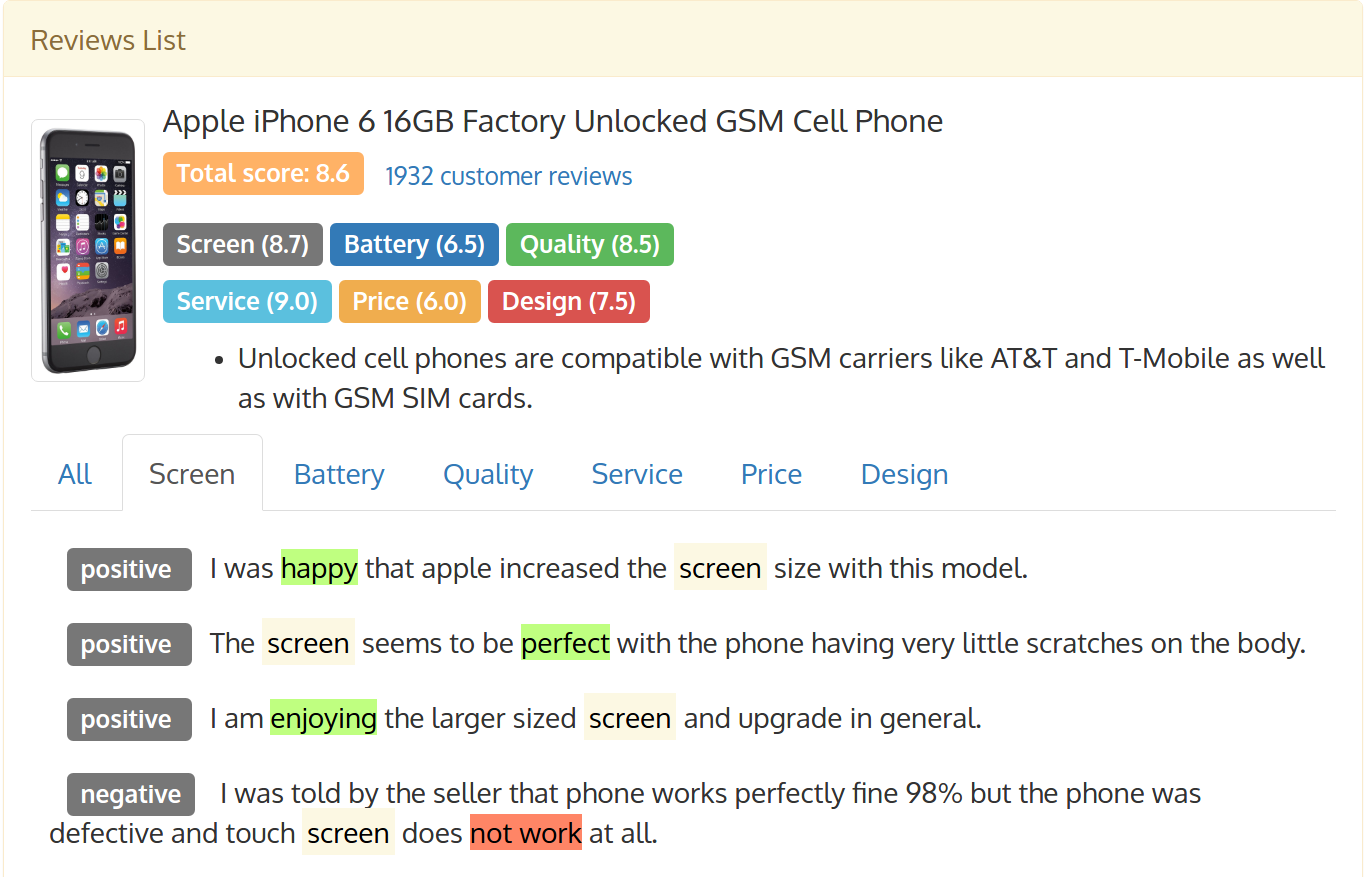
\includegraphics[width=\columnwidth]{figures/sentimentexample.png}}
%	\caption{Review snippets displayed by the aspects\label{fig:experiments:sentimentexample}}
%\end{figure}
%
